% Chapter Template

\chapter{Conclusions} % Main chapter title

\label{Chapter5} % For referencing this chapter elsewhere, use \ref{Chapter5}

%----------------------------------------------------------------------------------------
%	SECTION 1
%----------------------------------------------------------------------------------------

In the context of autonomous distributed satellite missions, new architectures and innovative control systems are still under exploration. The challenges presented by these distributed systems have to be solved to enable the migration from monolithic platforms to more complex architectures. Distributed on-board Mission Planning Systems are a key element of such satellite missions. As one of the core elements of these autonomy systems, distributed task scheduling policies are studied and have been the main focus of this thesis.

In this work the Local-Global policy has been completely designed and implemented. An appropriate state-of-the-art system has also been implemented for comparing and testing the performance of the Local-Global policy. The parameters for the comparison have been defined and large testing benchmarks have been performed for both algorithms, quantitatively measuring the behaviour of each one of them. All these results have to be analysed to obtain relevant conclusions about the development of the Local-Global policy and the future work to be done.

\section{Analysis of the results and the quality of the solutions}

The most significant results have been shown in chapter \ref{Chapter4}. However, some particularities of each algorithm that cannot be observed in those figures have to be explained and need to be commented in order to properly understand the advantages and disadvantages of each algorithm.

To begin with, it is important to note that the Local-Global policy considers several quality parameters in its optimization process: not only does it consider the amount of scheduled tasks, but also the associated resource consumption, the eagerness of the system to serve the requests, its responsiveness and utility (see definition of $F$ in section \ref{sec_F_LG}). Moreover, the tasks can be scheduled concurrently and any resource definition can be introduced in the problem definition. Finally, the golden index can be optimized for each satellite, either statically or dynamically by the \emph{Global} instance. This is not the case for the price-based algorithm which does not present such characteristics. This can model much better the heterogeneity among the satellites. In fact, homogeneity in the system deteriorates the results of the Local-Global, as very similar sub-solutions are delivered to the \emph{Global} from several satellites, restricting the number of chances to find a good solution.

The price-based scheduler, on the other hand, also has some characteristics that are not found on Local-Global: dependence between tasks and its resulting communication cost (passing the results of a task from one satellite to another) is considered during the schedule generation. Furthermore, the market model allows to include new features in the bid calculation which could take into account other system characteristics. Such redefinition of the bid could be done statically or dynamically.

When both algorithms are compared, it can be observed that the price-based execution times and memory usage are lower than those of the Local-Global, but there are some characteristics to be noted: while the price-based sequential nature of the scheduling process is a bottleneck and causes a saturation point that decreases the performance for high number of input tasks (Fig. \ref{fig_aMB}), the Local-Global's saturation is softer and it achieves to maintain the number of scheduled tasks for this situation (Fig. \ref{fig_aLG_alim}). The price-based scheduler also requires good communication among the satellites forming the cluster, a condition which could be hard to satisfy in a highly-constrained bandwidth context such as the open space. %The Local-Global's poor performance for high values of number of satellites and golden index can be improved by optimizing the \emph{Local} entity and smartly adapting the values of the golden index.
Noteworthy, the Local-Global performance is strongly affected by the performance of the local entity, as it can be seen in the results for large sets of satellites and high $\Delta$'s (see Fig. \ref{fig_tmLG_slim}). Redefining the current search heuristics of local schedulers, which have not been optimized and are not efficient in the current study, could improve, significantly, the overall performance of the L-G scheduler (Fig. \ref{fig_local_global}).

\begin{figure}[h!]
  \begin{minipage}[b]{\linewidth}
    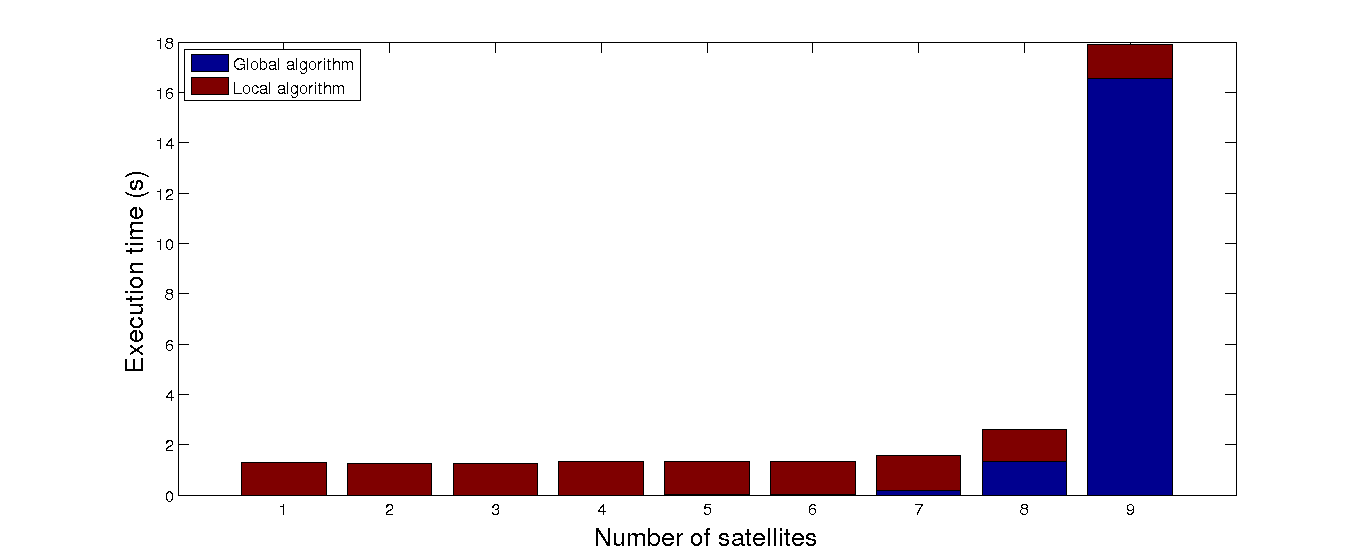
\includegraphics[width=\linewidth]{Figures/local_global.png}
    \caption{%
Local-Global: execution time differentiating the Local and the Global algorithms (varying number of satellites)} % End of caption
\label{fig_local_global}
  \end{minipage}
  \end{figure}

For these simulations $\Delta$ has been fixed to 5 and the number of input tasks is of 15. Note that for lower numbers of satellites (i.e. less than 8), the performance figure is dominated by the computation time of $\Delta_i$ local sub-solutions, while for cases in which the constellation has more than 8 satellites, the performance of the policy is dominated by the behaviour of the \textit{Global} algorithm.

\section{Future work}

As a core part of a Mission Planning System for distributed satellite missions, this thesis has developed a distributed task scheduler based on the of the Local-Global policy presented in \cite{Araguz15}. The results obtained allow to identify future strands of work for the Local-Global policy:

\begin{itemize}
\item The local algorithm has not been designed to search the solution space efficiently. Instead, the local scheduler randomly generates possible sub-solutions that fit the resource constraints. Moreover, the local scheduler does not provide sub-solutions in decreasing order (i.e. those with better $F$ first, and those with worse $F$ later). In fact, it does not even provide the best set of sub-solutions (i.e. the most optimal ones) but just the $\Delta$ first. 

Although this behaviour was sufficient for the sake of the analysis performed in this thesis, it actually worsens the quality of the global solution and negatively affects the overall performance. That being said, this situation clearly identifies an important improvement for this policy which lays beyond the scope of this thesis.

%\item Although the current performance can be deemed reasonably good as a first approach, an improvement can be obtained by optimizing the \emph{Local} scheduler. This importance of the \emph{Local} scheduler comes from the fact that it is the algorithm that generates the sub-solutions to be combined by the \emph{Global}: to find the optimal combination of sub-solutions, the set of available sub-solutions has to be of high quality and as heterogeneous as possible.

%The optimization of this scheduler should be done on the sub-solutions generation: although each sub-solution, if considered on its own, is a good result, obtained in very low time, the whole set of $\Delta_i$ sub-solutions are not optimal, as they may not be the best sub-solutions to be found, and they may contain repetitions among them.

\item On the other hand, some optimizations could be implemented for the \emph{Global} combinatorial search. Despite having very good performance when the constellation is composed of heterogeneous satellites, it decreases dramatically for homogeneous cases. These cases need to be studied in detal in order to further improve the algorithm.

\item In order to adapt better to heterogeneous systems with satellites which greatly differ in computational capabilities, a dynamic control on the golden index value for each satellite should be designed and implemented.

\item Implementing the Local-Global policy in a hierarchical system would allow to explore the scalability in cornerstone scenarios (e.g. constellations with hundreds of satellites). A modified version of the system that could group the satellites in small clusters (with different cluster generation approaches) would allow to explore new system features and situations where local algorithms may perform even better (e.g. clusters with specialized satellites each member would only schedule tasks for what it has been designed for, thus reducing the complexity of the local problem).

\item Task dependence defined in the price-based scheduler could be included in the policy, as it is a practical functionality to be implemented for small tasks forming an entire mission or activity.

\item The presented algorithm requires a single point of communication during the scheduling phase,a situation that can be slightly unrealistic in some scenarios. A more constrained communication model should be implemented to see how this affects the Local-Global performance (with a communication model similar to that of \cite{bonnet2008coordination}).
\end{itemize}